Currently, ATLAS deploys 20 instances of PanDA Broker on 4 Titan's DTNs, 5
instances per DTN. Each broker submits and manages the execution of 15 to 300
detector simulation jobs, one job for each work node, and a theoretical maximum
concurrent use of 96,000 cores. Since November 2015, PanDA Brokers have operated
only in backfill mode, without a defined time allocation, and running at the
lowest priority on Titan.

We evaluate the efficiency, scalability and reliability of the PanDA Brokers
along two dimensions: (i) the amount of backfill availability utilized by the
PanDA Brokers; and (ii) the amount of % job walltime
runtime spent performing detector simulations. \jhanote{it is difficult to parse
what (ii)?}\mtnote{Better?} We based these evaluations on measuring the number
of cores utilized by ATLAS on Titan, the overall backfill availability, the
number of detector simulations performed on all the resources available to ATLAS
and on Titan, and the failure rate of these simulations. All the measurements
were performed between January 2016 and February 2017.

% -----------------------------------------------------------------------------
\subsection{Utilization and Efficiency of PanDA Broker on Titan}
\label{ssec:panda_titan}

Figure~\ref{fig:core-hours-utilization} shows the number of core-hours used by
ATLAS on Titan, from January 2016 to February 2017. During that period, ATLAS
consumed a total of 73.8M core-hours, for an average of $\approx$ 7M core-hours a month,
with a minimum of 3.3M core-hours in April 2016 and a maximum 14.8M core-hours
in February 2017.

% \begin{figure}[htp]
%     \subfloat[]{
%         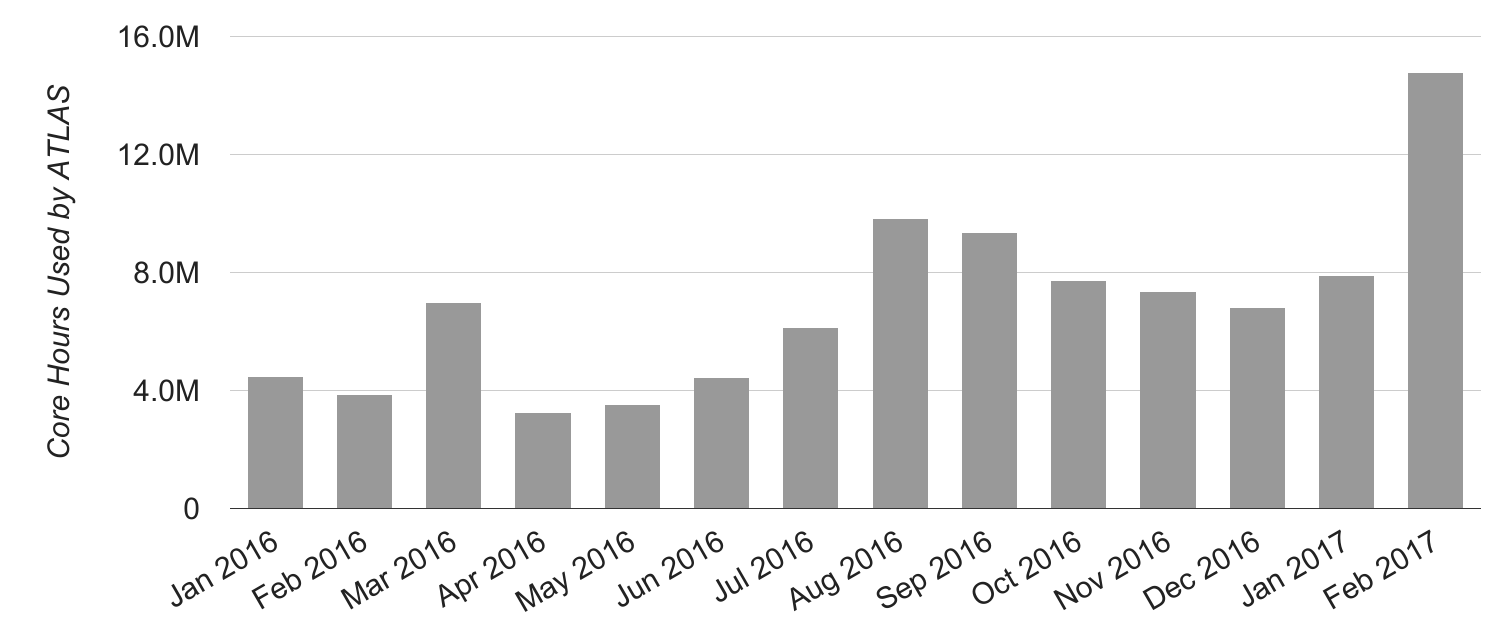
\includegraphics[clip,width=\columnwidth]{figures/cpu_hours.png}
%         \label{fig:core-hours-utilization}
%     }
%
%     \subfloat[]{
%         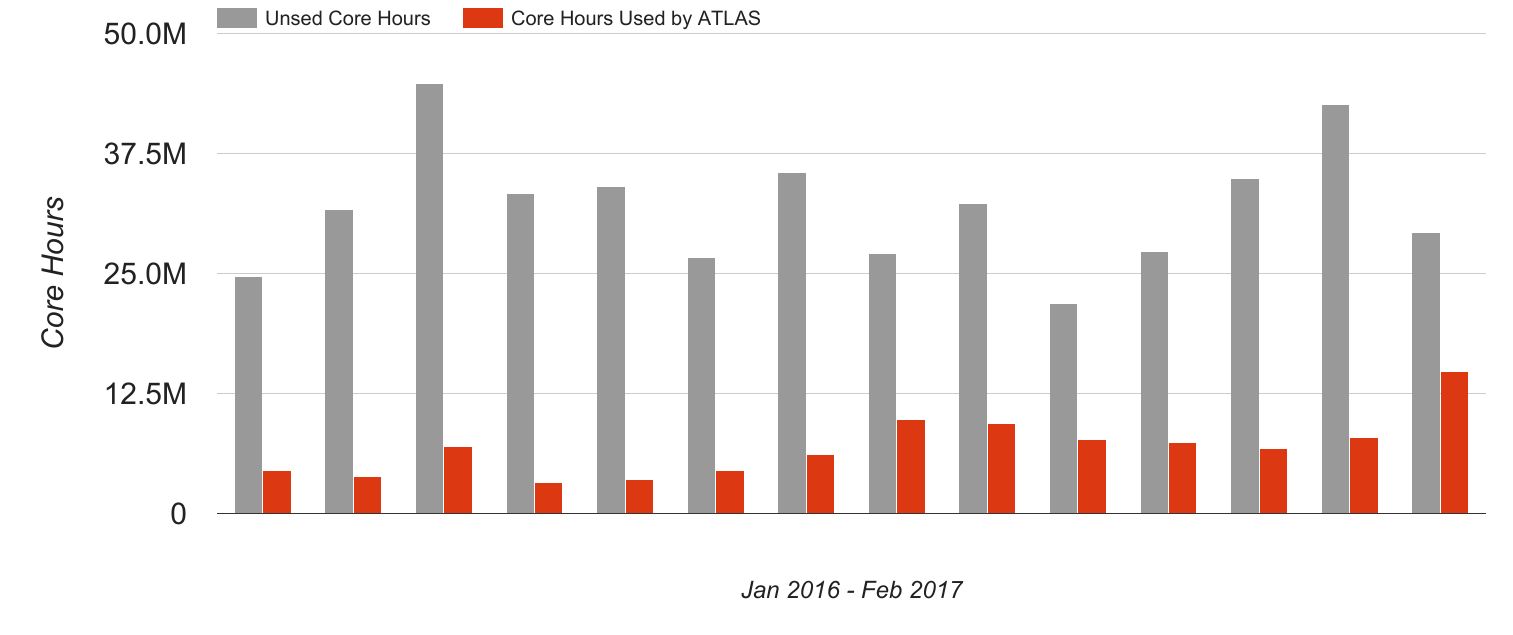
\includegraphics[clip,width=\columnwidth]{figures/backfill_consumption.png}
%         \label{fig:backfill-utilization}
%     }
% \caption{(a).(b).}
% \end{figure}

\begin{figure}[htp]
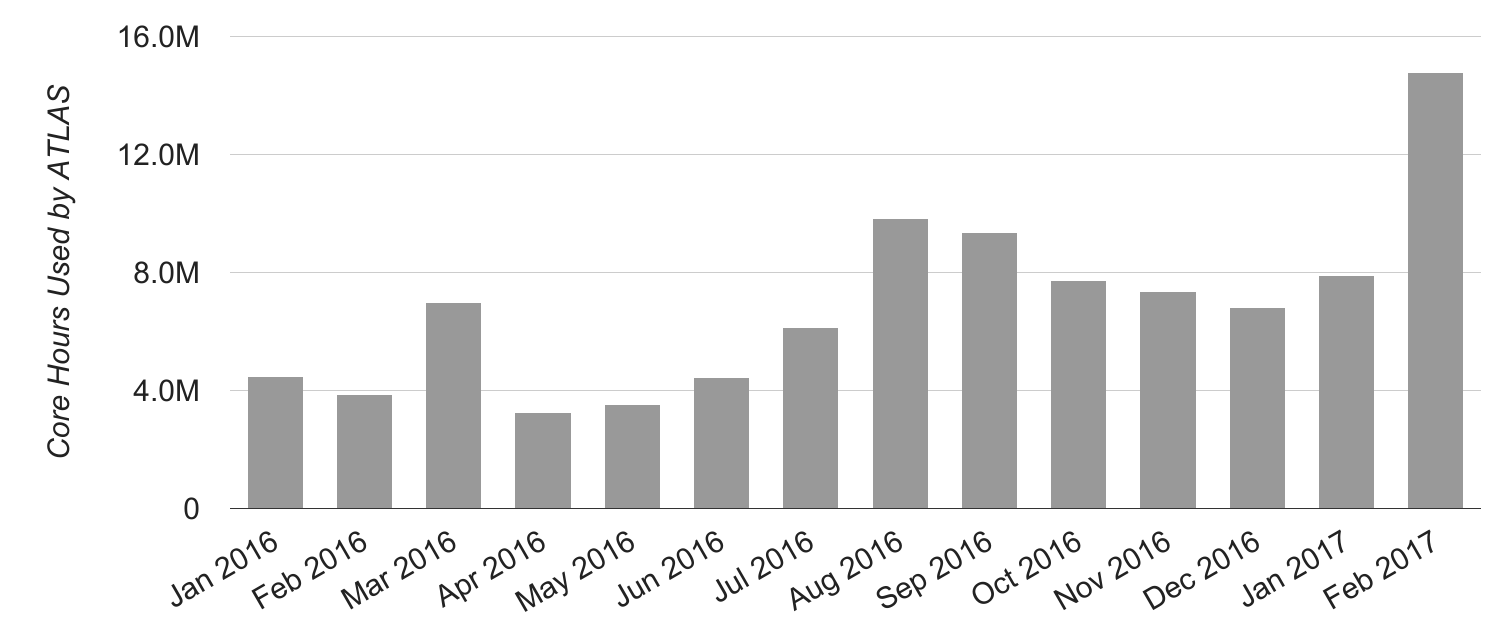
\includegraphics[clip,width=\columnwidth]{figures/cpu_hours.png}
\caption{Caption.}
\label{fig:core-hours-utilization}
\end{figure}

Figure~\ref{fig:backfill-utilization} shows backfill utilization from January
2016 to February 2017. \jhanote{Neither figure show efficiency. Both show
utilization.} Efficiency is defined as the fraction of Titan’s cores available
via backfill that was utilized by the PanDA Brokers. \jhanote{I would plot the
efficiency on the Y2 axis for both.} The brokers reached 18\% average efficiency
\jhanote{this sentence is a bit difficult to parse. Is the 18\% overall
efficiency?}\mtnote{average across all months considered. Should I call it
``overall''?} with a minimum 8.9\% efficiency on April 2016 and a maximum 33.5\%
efficiency on February 2017. The number of total backfill cores available was
38.1M in April 2016, and 33.1M in February 2017. This shows that the measured
difference in efficiency did not depend on a comparable difference in total
backfill availability.

\begin{figure}[htp]
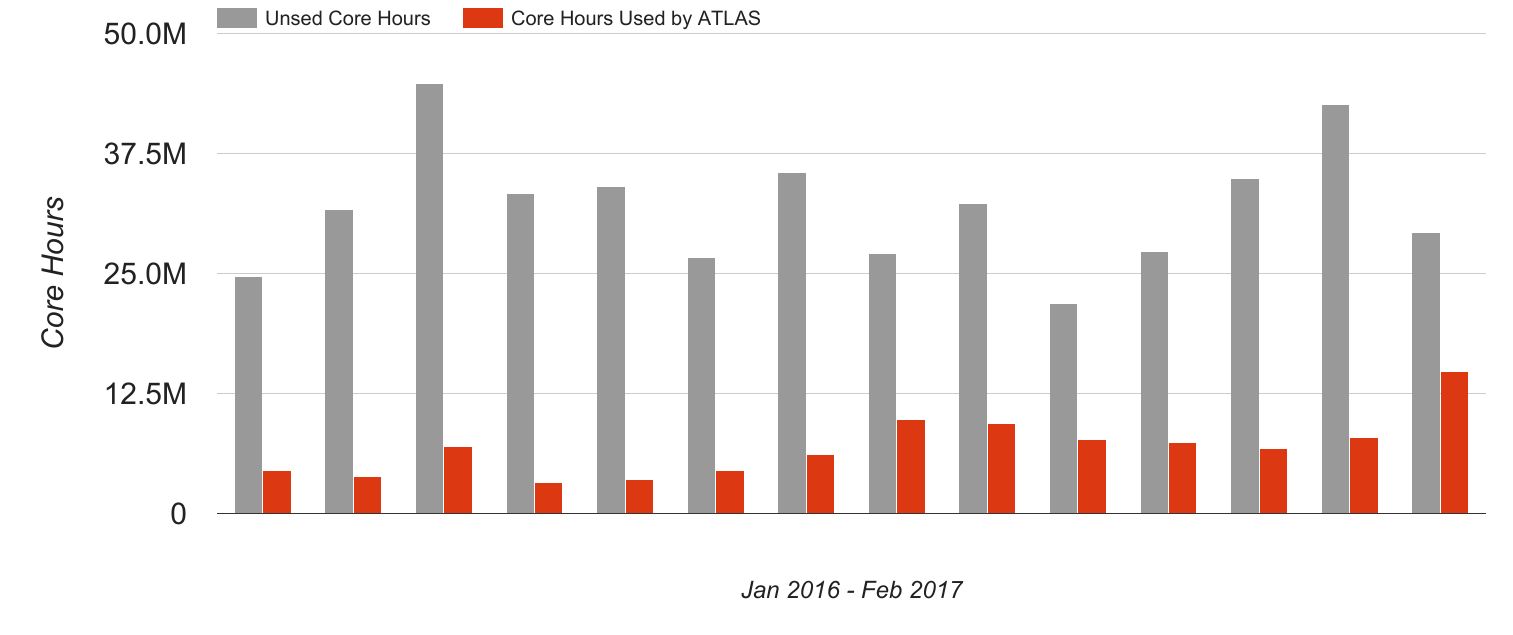
\includegraphics[clip,width=\columnwidth]{figures/backfill_consumption.png}
\caption{Caption. \jhanote{I would suggest similar style of X-axis as previous figure. Difficult to parse which is April if we are going to call out a specific month. Also consistency in style is generally good to keep cognitive burden low.}}
\label{fig:backfill-utilization}
\end{figure}

Figure~\ref{fig:hpc-workload-utilization} shows that between January 2016 and
February 2017, about 2.25M detector simulation jobs were completed on Titan, for
a total of 225M events processed. This is equivalent to 0.9\% of all the 250M
detector simulations performed by ATLAS in the same period of time, and 3.5\% of
the 6.6B events processed by those jobs. Comparatively, Titan contributed 3.9\%
of the total of around 200K cores available to ATLAS on Grid, Cloud, and HPC
infrastructures together. These figures confirms the relevance of
supercomputers' resource contribution to the LHC Run 3, especially when
accounting for the amount of unused backfill availability and the rate of
improvement of PanDA efficiency.

\begin{figure}[htp]
    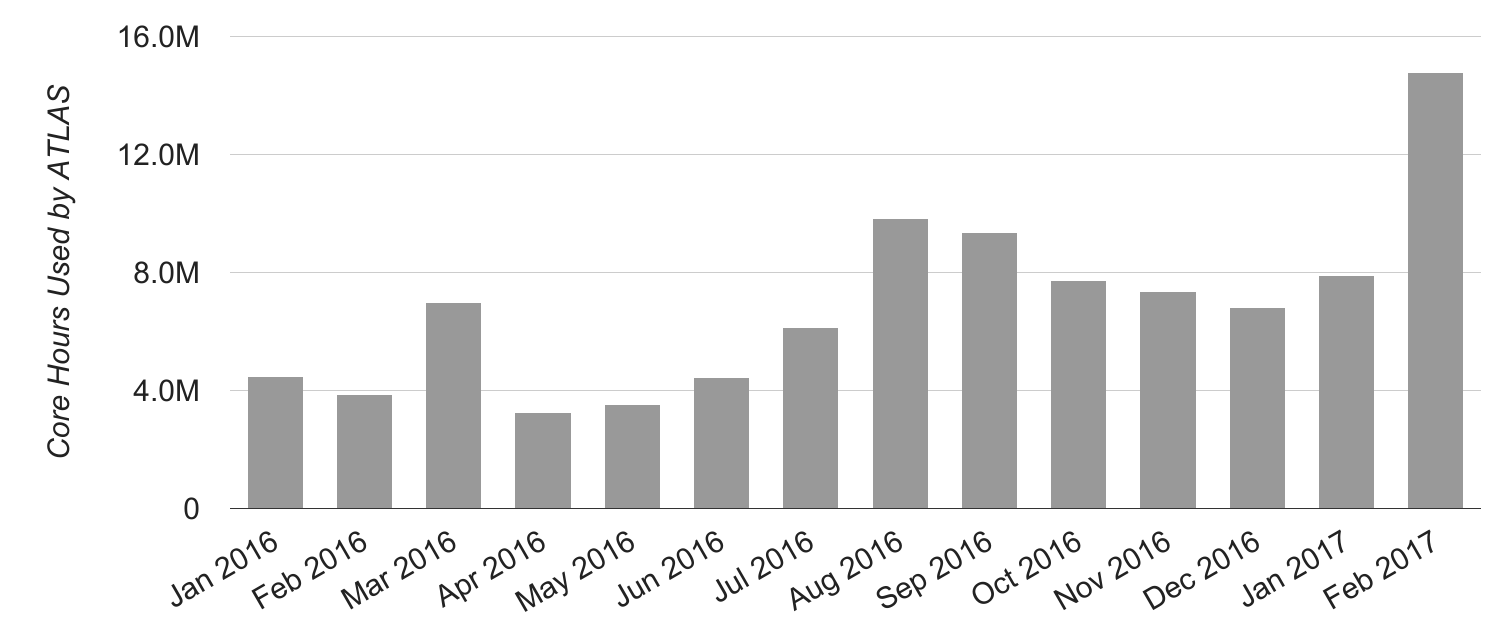
\includegraphics[clip,width=\columnwidth]{figures/cpu_hours.png}
\caption{\mtnote{Placeholder for the diagram/data I asked to Danila and
Sergey. Consider a table instead of a figure.}}
\label{fig:hpc-workload-utilization}
\end{figure}

On February 2017, PanDA Brokers used almost twice as much backfill availability
than in any other month. No relevant code update was made during that period and
logs indicated that the brokers were able to respond more promptly to backfill
availability. This is likely due to hardware upgrades on the DTNs. The absence
of continuous monitoring of the nodes does not allow to quantify bottlenecks but
spot measurements of the DTNs load indicate that a faster CPU and better
networking were likely responsible for the improved performance.

Investigations showed an average CPU load of 3.6\% on the upgraded DTNs. As
such, further hardware upgrades seem unlikely to improve significantly the
performance of PanDA Brokers. Nonetheless, the current load suggests that the
number of brokers per DTN could be increased. This would enable the submission
of a larger number of concurrent jobs to Titan's PBS queue, allowing for PanDA
to consume a higher percentage of backfill availability.


All the detector simulations executed on Titan process 100 events. This number
has been chosen by observing the average walltime of backfill resources: too
many events would \ldots\mtnote{I need to speak further to Sergey to clarify
this.}.

Usually, detector simulations performed on the Grid process a higher number of
events than those on Titan. This explains the difference between the percentage
of detector simulations (9\%) and of events computed by those simulations
(3.9\%) on Titan. PanDA Event Service~\cite{panda-event-service} will contribute
to address this limitation: each PanDA Broker will be able to pull a variable
number of events for each simulation, depending on the available walltime. This
functionality is currently being implemented.

Given the current design and implementation, the utilization of a larger portion
of Titan's backfill availability depends on the the number of concurrent PanDA
Brokers instantiated on the DTNs.
% The number of concurrent detector simulation jobs that PanDA Broker can manage
% depends on the DTNs' resources. Each PanDA Broker can execute 1 MPI PBS job on
% up to 300 work nodes for a total of 4,800 cores. Scaling above this threshold
% requires instantiating multiple PanDA Brokers on the same DTN and, once the
% DTN resources are saturated, on multiple DTNs.
In principle, this is not a problem on Titan as multiple DTNs are supposed to be
available and periodically upgraded. Assuming the efficiency reached on February
as reference, using all the available backfill resources on Titan would require
around 60 concurrent PanDA Brokers. Further testing and better monitoring
capabilities are required to establish whether the current DTN capabilities can
support this load, especially when considering the increased volume of files
staged in and out the DTNs.

\mtnote{Extend/change previous paragraph explaining also the problem of the
`spike'/`wave' of backfill availability. The problem without enough brokers to
cope with variable amounts of backfill availability is that we may exhaust all
20 brokers to use a portion of backfill smaller than the one that becomes
available when no more brokers are available.}

% -----------------------------------------------------------------------------
\subsection{Efficiency and Scalability of Detector Simulation on Titan}
\label{ssec:panda_titan}

\begin{itemize}
    \item problem with lustre addressed with ramdisk
    \item Competition for cache in AMD processors.
    \item Summary overall figure of performance analogous to those produced with NGE. Diagram as discussed in F2F meeting at Rutgers.
    \item Comparison hardware performance Titan/Grid
\end{itemize}

We use two main parameters to measure the performance of the detector simulation
jobs submitted to Titan: (i) the time taken to setup
AthenaMP~\cite{aad2010atlas}, the ATLAS software framework integrating the
GEANT4 simulation toolkit~\cite{agostinelli2003geant4}; and (ii) the
distribution of the time taken by the Geant4 toolkit to simulate a certain
number of events.

AthenaMP has an initialization and configuration stage. At initialization time,
AthenaMP is assembled from a large number of shared libraries, depending on the
type of payload that will have to be computed. Once initialized, every algorithm
and service of AthenaMP is configured by a set of Python scripts. Both these
operations result in a large number of read operations on the filesystem,
including those required to access of small python scripts.

% AthenaMP is a multipurpose framework that needs to be configured depending on
% the type of payalod that needs to be executed. For Geant4, this configuration
% process links up to 200 libraries, all requiring filesystem read and write
% operations.

% The execution of Geant4 is mostly compute-intensive requiring to write around
% XXKB per 100 events on disk and no more than 2GB of memory.

% -----------------------------------------------------------------------------
% \subsection{PanDA Shared Library I/O Performance Impact at OLCF}

% Athena, the ATLAS framework has a configuration and initialization stage. At
% this stage, the running job is assembled on the fly from a large number of
% shared libraries. Also, at this stage, every algorithm and service is being
% configured, at run time, by a corresponding set of Python scripts, which
% results in a large number of read operations accesses to small python
% scripts, with many includes and imports Python calls.

Initially, all the shared libraries of AthenaMP and the python scripts for the
configuration stage were stored on the Spider 2 Lustre file system. However, the
I/O patterns of the initialization and configuration stages degraded the
performance of the filesystem (Figure~\ref{}\mtnote{We may want to aggregate
some of the diagrams about lustre's experiments here}). Since Spider 2 is a
center-wide file system, this resulted in  performance degradation for all OLCF
resources and users. \mtnote{I am afraid the details about the trace are too
specific given the space constraints of a SC submission. Please feel free to
uncomment it if you disagree.}
% As can be seen in Listing~\ref{mdstrace} the metadata I/O activity for ATLAS
% exhibits a spike corresponding to the beginning of the runs before tapering
% off.

% \begin{minipage}{\linewidth}
% \begin{lstlisting}[language=bash,frame=single,basicstyle=\ttfamily\tiny,caption=ATLAS metadata trace,label=mdstrace]
% XK7 Application 9205593
%       39012 RPCs from 300 of 300 nodes
%         ~69291.96 per sec
%           37851 LDLM_ENQUEUE RPCs    ~67229.83 per sec
%                 pmin 13us pavg 42us pmax 4983us
%           611 LDLM_CANCEL RPCs    ~1085.24 per sec
%                 pmin 10us pavg 16us pmax 32us
%           277 MDS_CLOSE RPCs    ~492.00 per sec
%                 pmin 15us pavg 20us pmax 38us
%           154 MDS_READPAGE RPCs    ~273.53 per sec
%                 pmin 170us pavg 292us pmax 671us
%           86 MDS_GETXATTR RPCs    ~152.75 per sec
%                 pmin 15us pavg 21us pmax 65us
%           30 MDS_GETATTR RPCs    ~53.29 per sec
%                 pmin 16us pavg 20us pmax 27us
%           3 MDS_REINT RPCs    ~5.33 per sec
%                 pmin 103us pavg 136us pmax 196us
%           Overall times
%                 pmin 10us pavg 42us pmax 4983us
%
% XK7 Application 9205355
%       8698 RPCs from 62 of 62 nodes
%         ~15449.13 per sec
%           8445 LDLM_ENQUEUE RPCs    ~14999.76 per sec
%                 pmin 16us pavg 41us pmax 780us
%           92 MDS_CLOSE RPCs    ~163.41 per sec
%                 pmin 15us pavg 23us pmax 52us
%           55 MDS_READPAGE RPCs    ~97.69 per sec
%                 pmin 189us pavg 291us pmax 534us
%           52 LDLM_CANCEL RPCs    ~92.36 per sec
%                 pmin 12us pavg 16us pmax 25us
%           41 MDS_GETXATTR RPCs    ~72.82 per sec
%                 pmin 16us pavg 20us pmax 27us
%           13 MDS_GETATTR RPCs    ~23.09 per sec
%                 pmin 16us pavg 21us pmax 38us
%           Overall times
%                 pmin 12us pavg 42us pmax 780us
%
% \end{lstlisting}
% \end{minipage}

% As this problem was identified, the OLCF staff has enabled read-only access to
% certain NFS-exported directories from Titan compute nodes. This in turn
% allowed the OLCF staff to install a software package from a Titan login node
% and have it available read-only on a Titan compute node.

After careful characterization of the impact of ATLAS jobs on Lustre, the
performance degradation was addressed by moving the AthenaMP distribution to a
read-only NFS directory, shared among DTNs and work nodes. This eliminated the
problem of metadata contention, improving metadata read performance from \~6,300
seconds on Lustre to \~1,500 seconds on NFS. Further, at configuration time, the
input files of each detector simulation job were stored to a ramdisk on the work
nodes. This offered a marked improvement of reading time: from 1,320 seconds on
Lustre to 40 seconds on NFS.

%Figure~\ref{fig:atlas-perf-improvement} shows the overall ATLAS performance
%improvement on Titan. The circled region illustrates the switch from Lustre to
%NFS-exported directory for hosting the ATLAS release.

%\begin{figure}[!htb]
%    \centering
%    \begin{tabular}{cc}
%        {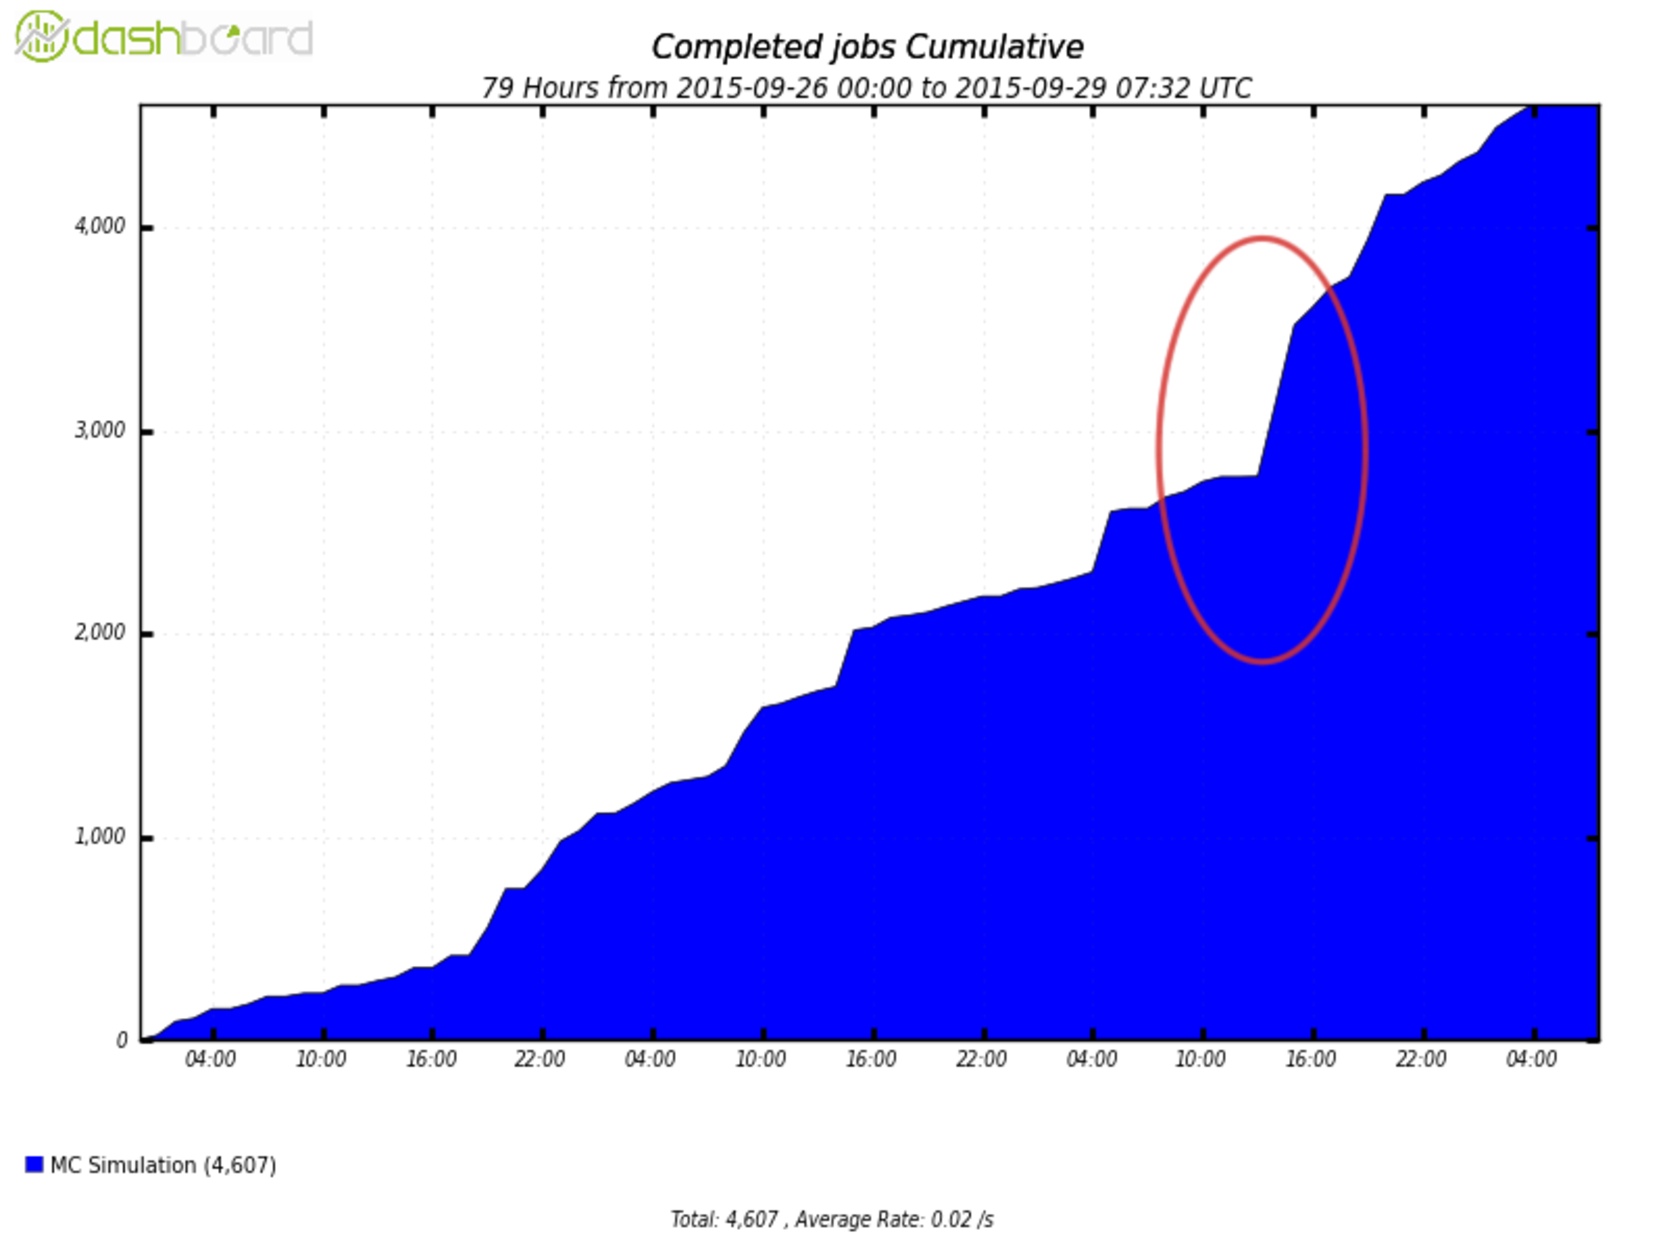
\includegraphics[width=0.48\textwidth]{figures/panda-completed-jobs-sw-move.pdf}}\\
%    \end{tabular}
%    \caption{ATLAS performance improvement on Titan. The circled region shows the switch from Lustre to NFS-exported directory for hosting the ATLAS release.}
%\label{fig:atlas-perf-improvement}
%\end{figure}

At runtime, detector simulation jobs showed performance degradation when all the
16 cores of Titan's work nodes were used. As shows in
Figure~\ref{}\mtnote{Sergery: do you have a diagram showing the difference in
performance between using 16 and 8 cores for a detector simulation job with 100
events?}, the mean runtime for 8 concurrent jobs computing 100 events is XXXs,
with each job executed in 8 distinct processes, one per core. The mean runtime
for 16 concurrent jobs computing 100 events is instead XXXs. This can be
explained by looking at the cache architecture of the AMD Opteron 6274 CPU. In
this processor, every two cores share the level 1 instruction cache, impacting
the performance of \ldots\mtnote{Do we kow what instruction set is affected?}
computation.

The compute performance of Titan for detector simulation jobs is, on average,
lower that that of LCWG. Figure~\ref{}\mtnote{Sergey: I remember you showed us
some plots comparing Geant4 simulation's performance on Titan and some of the
Grid sites. Could we use one or two of the here?} shows the difference in
execution time of the same type of simulation between Titan and
\ldots\mtnote{Add the name of the grid sites here}. This is not an issue with
the design of PanDA Brokers and, more in general, with the migration of part of
the ATLAS workload to supercomputers: Titan has been active since 2012 and more
modern CPUs are expected to offer better performance. A pilot project is already
in place to test PanDA Broker on Summit, the next generation supercomputer that
will become active in 2018 at OLCF.

% ----------------------------------------------------------------------------
\subsection{Reliability of PanDA Broker and Detector Simulations on Titan}
\label{ssec:reliability}

The current design and architecture of the PanDA Broker is proving to be as
reliable as PanDA Pilot when used on the WLCG. Between Jan 2016 and Feb 2017,
the overall failure rate of all the ATLAS detector simulation jobs was 14\%,
while the failure rate of jobs submitted to Titan was a comparable 13.6\%. PanDA
Brokers were responsible for around the 19\% of the failures, compared to the
29\% of failures produced by the JobDispatcher module of the PanDA Server, and
the 13\% failures produced by the Geant4 toolkit. The current failure rate of
the PanDA Brokers confirms the benefits of reusing most of the code base of the
PanDA Pilot for implementing the PanDA Broker. It also shows that adopting
third-party libraries like RADICAL-SAGA did not have a measurable adverse effect
on reliability.

Figure~\ref{fig:failures-titan} shows a breakdown of the type of failures
recorded by the PanDA Brokers between January 2016 and February 2017. The
initial preponderance of unknown failures was progressively addressed by a more
accurate failure model, specifically tailored to the PanDA Broker and Titan. It
also shows the progressive improvement of the broker's reliability: In Februrary
2017, most of the failures were produced by the initialization and configuration
phases of AthenaMP or by failed executions of the payload.\mtnote{If we want to
keep this diagram, we will need to plot it from the CSV to make it readable.}

\begin{figure}[htp]
    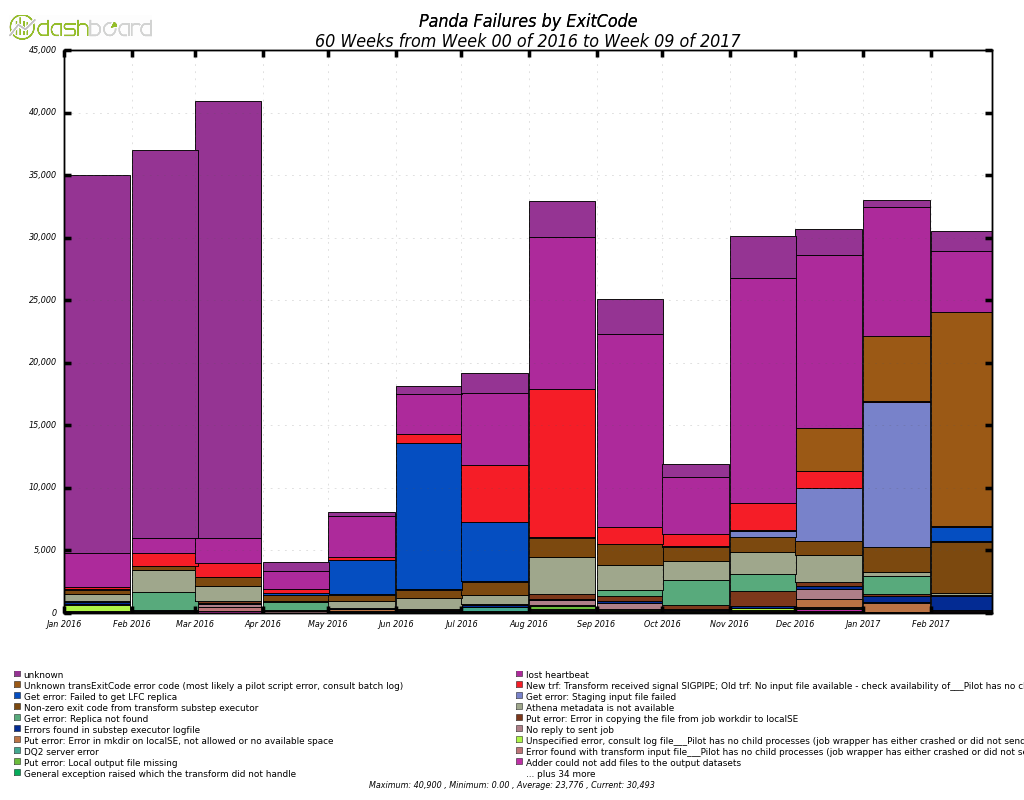
\includegraphics[clip,width=\columnwidth]{figures/failures_titan.png}
\caption{Caption.}
\label{fig:failures-titan}
\end{figure}


% -----------------------------------------------------------------------------
\subsection{PanDA I/O Impact at OLCF}

To better understand the I/O impact of ATLAS PanDA project on Titan
supercomputing environment we analyzed 1,175 jobs ran on the week of 10/25/2016,
for a total of 174 hours. Table~\ref{panda-olcf-stats} shows the overall
statistical breakdown of the observed file I/O impact of ATLAS at OLCF\@.
Figures~\ref{fig:atlas-titan-io-read} and~\ref{fig:atlas-titan-io-written} show
the file read and write I/O histograms for these 1,175 jobs, respectively.
Figures~\ref{fig:atlas-titan-file-open} and~\ref{fig:atlas-titan-file-close}
show the file $open()$ and $close()$ metadata load histograms of the same 1,175
ATLAS jobs, respectively.

As can be seen from Table~\ref{panda-olcf-stats}, the number of nodes used by
ATLAS jobs vary between 1 and 300, while the average is at 35. 75\% of the ATLAS
jobs consume less than 25 and 92\% consume less than or equal to 100 Titan
compute nodes. During the 174 hours of data collection, we observed that 6.75
ATLAS jobs were executed on average per hour on Titan and ran for 1.74 hours on
average.

ATLAS jobs issues a large number of file read operations, as can be seen in
Table~\ref{panda-olcf-stats}. The maximum amount read by any ATLAS job in
aggregate in this observed period was less than 250 GB and the maximum amount
written in aggregate was less than 75 GB\@. The average amount read per job is
20 GB and average amount written is 6 GB\@.

\begin{figure}[!htb]
    \centering
    \begin{tabular}{cc}
        {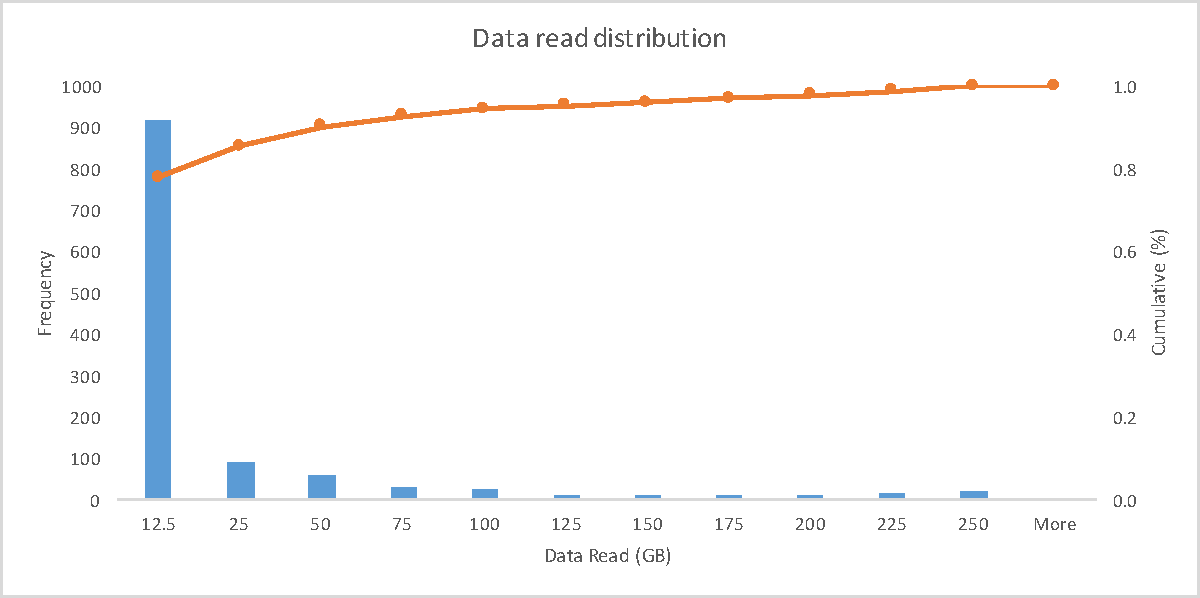
\includegraphics[width=0.48\textwidth]{figures/panda_data_read_finer_hist.pdf}}\\
    \end{tabular}
    \caption{ATLAS file read operation histogram on Titan for week of 10/25/16.}
\label{fig:atlas-titan-io-read}
\end{figure}

\begin{figure}[!htb]
    \centering
    \begin{tabular}{cc}
        {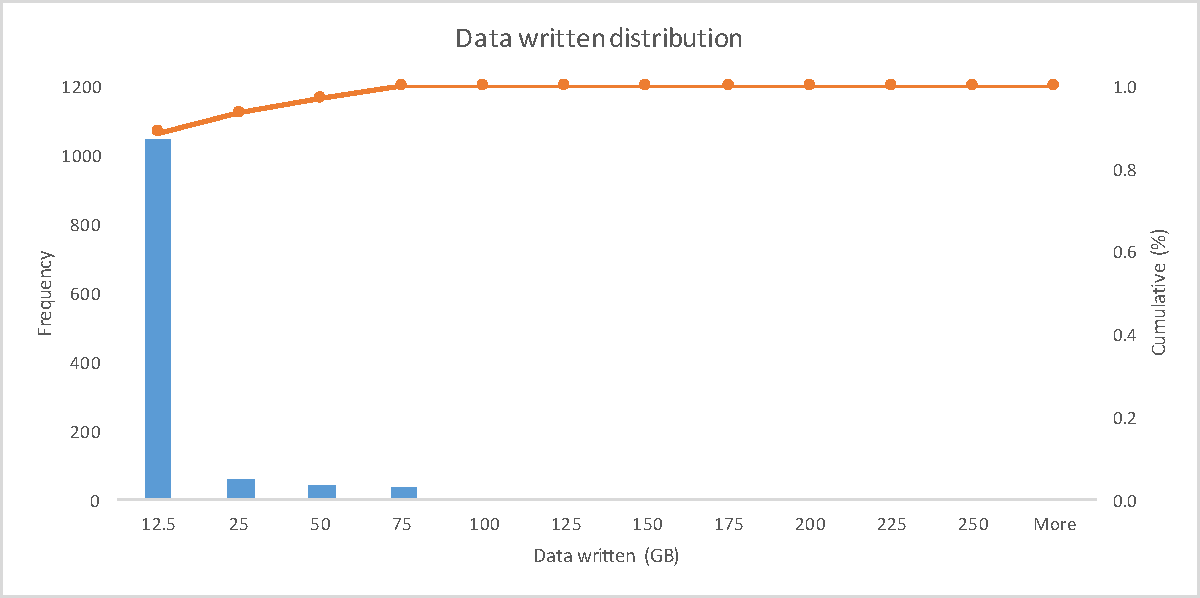
\includegraphics[width=0.48\textwidth]{figures/panda_data_written_finer_hist.pdf}}\\
    \end{tabular}
    \caption{ATLAS file write I/O histogram on Titan for week of 10/25/16.}
\label{fig:atlas-titan-io-written}
\end{figure}

Per job read and write file I/O statistics show an interesting pattern.
Table~\ref{panda-olcf-stats} indicates that the amount of data read per ATLAS
compute node on Titan is less than 400 MB on average, while the amount of data
written per node is less than 170 MB on average. This correlates with our
finding that ATLAS PanDA jobs are read heavy. However, as can be seen in
Table~\ref{panda-olcf-stats} and figures {fig:atlas-titan-io-read} and
{fig:atlas-titan-io-written}, the distribution between read and written amount
of data per job is quite different from one another. The read operation
distribution per job shows a long tail, ranging from 12.5 GB to 250 GB, while
the written amount of data has a very narrow distribution.

\begin{figure}[!htb]
    \centering
    \begin{tabular}{cc}
        {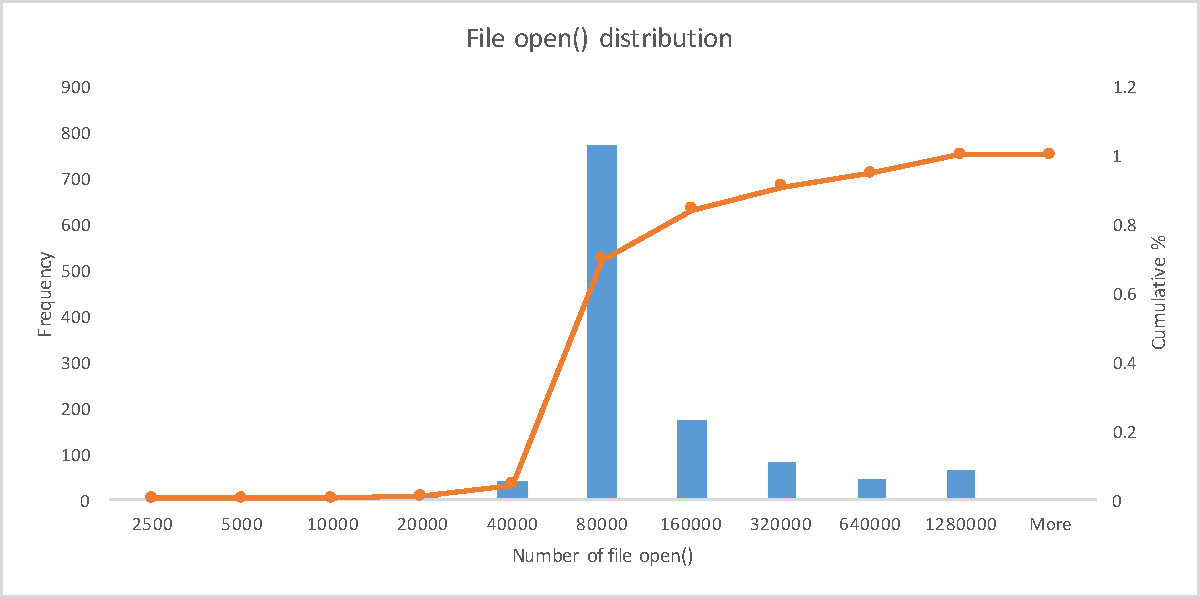
\includegraphics[width=0.48\textwidth]{figures/panda_file_open_hist.pdf}}\\
    \end{tabular}
    \caption{ATLAS file $open()$ histogram on Titan for week of 10/25/16.}
\label{fig:atlas-titan-file-open}
\end{figure}

\begin{figure}[!htb]
    \centering
    \begin{tabular}{cc}
        {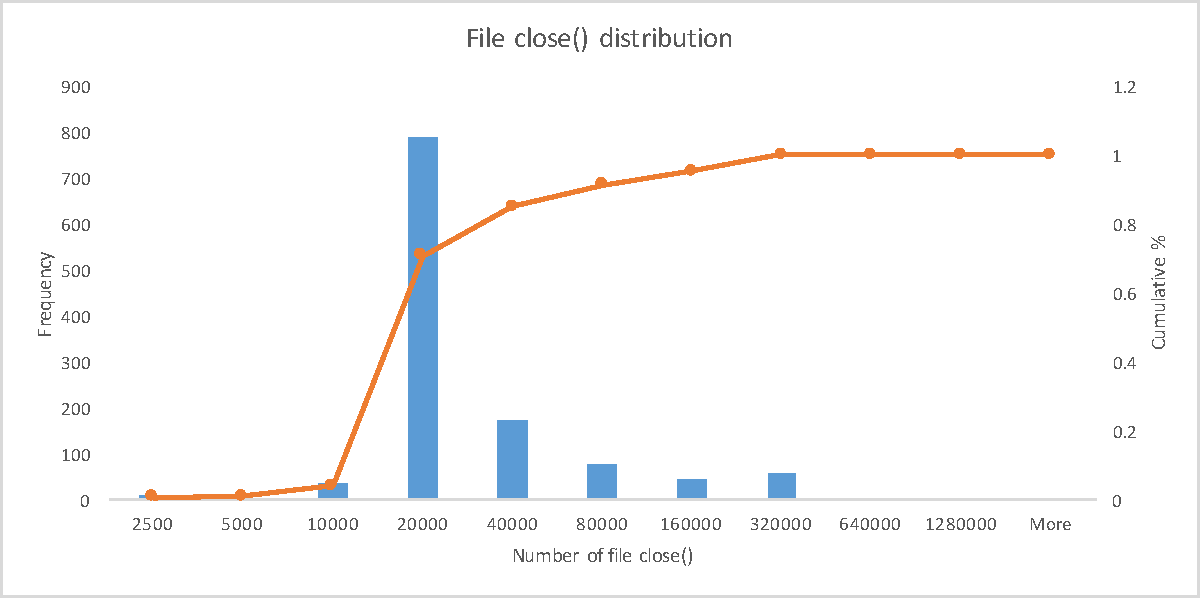
\includegraphics[width=0.48\textwidth]{figures/panda_file_close_hist.pdf}}\\
    \end{tabular}
    \caption{ATLAS file $close()$ histogram on Titan for week of 10/25/16.}
\label{fig:atlas-titan-file-close}
\end{figure}

On the metadata I/O breakdown, ATLAS PanDA jobs yield 23 file $open()$
operations and 5 file $close()$ operations per second. The file $open()$
operations listed here don't include the file $stat()$ operations. As can be
seen from figures~\ref{fig:atlas-titan-file-open}
and~\ref{fig:atlas-titan-file-close}, they exhibit similar distributions. The
maximum number of file $open()$ operations are around 170 on average and the
maximum number of file $close()$ operations are 39 on average per second per
job. The total number of file $open()$ operations is 172,089,760 for the
observed window of 174 hours, while the total number of file $close()$
operations stand at 40,132,992 for the total 1,175 ATLAS PanDA jobs in the same
observation window. The difference between these two values is puzzling and it
is under investigation at the time of writing this paper. One possible
explanation is that ATLAS PanDA jobs perhaps don't call a file $close()$
operation per every file $open()$ issued.

\begin{table*}[t]
\centering
\begin{tabular}{lllllllll}
 & Num. Nodes & Duration (s) & Read (GB) & Written (GB) & GB Read/nodes & GB Written/nodes & $open()$ & $close()$ \\
Min & 1 & 1,932 & 0.01 & 0.03 & 0.00037 & 0.02485 & 1,368 & 349 \\
Max & 300 & 7,452 & 241.06 & 71.71 & 0.81670 & 0.23903 & 1,260,185 & 294,908 \\
Average & 35.66 & 6,280.82 & 20.36 & 6.87 & 0.38354 & 0.16794 & 146,459.37 & 34,155.74 \\
Std. Dev. & 55.33 & 520.99 & 43.90 & 12.33 & 0.19379 & 0.03376 & 231,346.55 & 53,799.08
\end{tabular}
\caption{The Statistical breakdown of the I/O impact of 1,175 PanDA jobs executed at OLCF for the week of 10/25/16}
\label{panda-olcf-stats}
\end{table*}

Overall, based on our experiments with real-world jobs, it can be safely
concluded that the file and metadata I/O load of ATLAS PanDA project on the OLCF
Titan supercomputing environment and the Spider 2 file system is not detrimental
to the center operations and the overall impact is minimal, at the current scale
of the project.
